% Braking and destruction of a vortex by a weak magnetic field -- a letter.
%
% Build: make (in this directory). Every number below that comes from a run is
% printed by vd_numbers.py into vd_numbers.txt; the figures are made by
% figures.py (make figs). Formatted for Physical Review Letters with REVTeX 4.2.
%
% DRAFT, 2026-11-24. Every run is D3Q27 + D3Q7 with nz = 1: the map's
% Rm <= 4000, the slices, the controls and the frames were rerun on that lattice
% by GPU/csf3/vortex_disruption_d3q27.sub (results/Q_vortex_disruption/d3q27).
% The CUDA map's top rung (Rm = 32000, elements 32-39 of
% GPU/csf3/vortex_disruption_map.sub) was cancelled before it started, to be
% resubmitted: its registered rule over five rungs gives the verdict, and over
% the four here only an interim reading. When it lands: copy it into
% results/Q_vortex_disruption/gpu_campaign/map, `make -B`, and update the Rm
% range, p, U and Fig. 3.
\documentclass[aps,prl,twocolumn,reprint,amsmath,amssymb,superscriptaddress,floatfix]{revtex4-2}

\usepackage[utf8]{inputenc}
\usepackage[T1]{fontenc}
\usepackage{graphicx}
\usepackage{bm}
\usepackage[hidelinks]{hyperref}

\newcommand{\Rm}{\mathrm{Rm}}
\newcommand{\Rey}{\mathrm{Re}}
\newcommand{\eps}{\varepsilon}

\begin{document}

% Let the two column figures share a page with the full-width Fig. 1 and the
% text, instead of drifting to pages of their own after the references.
\renewcommand{\topfraction}{0.9}
\renewcommand{\bottomfraction}{0.9}
\renewcommand{\textfraction}{0.07}
\renewcommand{\floatpagefraction}{0.8}
\renewcommand{\dbltopfraction}{0.9}
\setcounter{topnumber}{3}
\setcounter{bottomnumber}{2}
\setcounter{totalnumber}{5}


\title{A weak magnetic field brakes a vortex as \texorpdfstring{$M^2\Rm^{2/3}$}{M2 Rm2/3} and destroys it as \texorpdfstring{$M^2\Rm$}{M2 Rm}}

\author{Alessandro De Rosis}
\email{alessandro.derosis@manchester.ac.uk}
\affiliation{The University of Manchester, Manchester M13 9PL, United Kingdom}
% TODO(author): department line.

\date{\today}

\begin{abstract}
A vortex winds a weak magnetic field into thin current sheets whose stresses can
destroy it. Whether that takes $M^2\Rm\sim1$ or $M^2\Rm^{2/3}\sim1$, with $M$ the
field in units of the flow speed and $\Rm$ the magnetic Reynolds number, has
remained open because simulations have spanned too narrow a range of $\Rm$.
Following one vortex over $\Rm=250$--$16\,000$ with two independent lattice
Boltzmann codes, we find both: the braking during the wind-up grows as
$M^2\Rm^{2/3}$, while destruction needs $M^2\Rm\approx2$, a field
$M_c\propto\Rm^{-0.50\pm0.06}$. At large $\Rm$ a weak field therefore destroys a
vortex that it has barely braked.
\end{abstract}

\maketitle

A vortex in a weak, uniform magnetic field winds the field lines up until
diffusion lets them reconnect; the field is then expelled from the core and
concentrated at its edge \cite{weiss1966}. During the wind-up the field is
amplified to $b\sim\Rm^{1/3}B_0$ on a scale $\Rm^{-1/3}$ of the vortex
\cite{weiss1966}, so at the large magnetic Reynolds numbers of astrophysical flows a
field far too weak to matter on the large scale can be dynamically important on the
small one. Such fields suppress turbulent transport \cite{cattaneo1991} and the
formation of jets in $\beta$-plane turbulence \cite{tobias2007}. For a single
vortex the question is how strong the field has to be to disrupt it, and two
answers have been given. Mak, Griffiths and Hughes \cite{mak2017} compared the curl
of the magnetic tension of the wound field with the inertia of the vortex and
obtained $M^2\Rm\sim1$, with $M$ the ratio of the Alfv\'en speed to the flow speed.
Gilbert, Mason and Tobias \cite{gilbert2016}, in a quasilinear model in which the
flow is held axisymmetric and the magnetic Prandtl number is small, found that the
Lorentz force takes over above
$b_0=O(U\Rm^{-1/3})$, that is at $M^2\Rm^{2/3}\sim1$. The simulations of
Ref.~\cite{mak2017} spanned $\Rm=50$--$1000$, and its authors noted that the two
scalings could not be told apart there. Tessier, Poulin and Hughes
\cite{tessier2025} have since mapped the regimes of vortex arrays as the field
grows, at one $\Rm$. The difference is not academic: at $\Rm=10^{12}$ the two
criteria differ by a factor $10^4$ in field energy.

\begin{figure*}
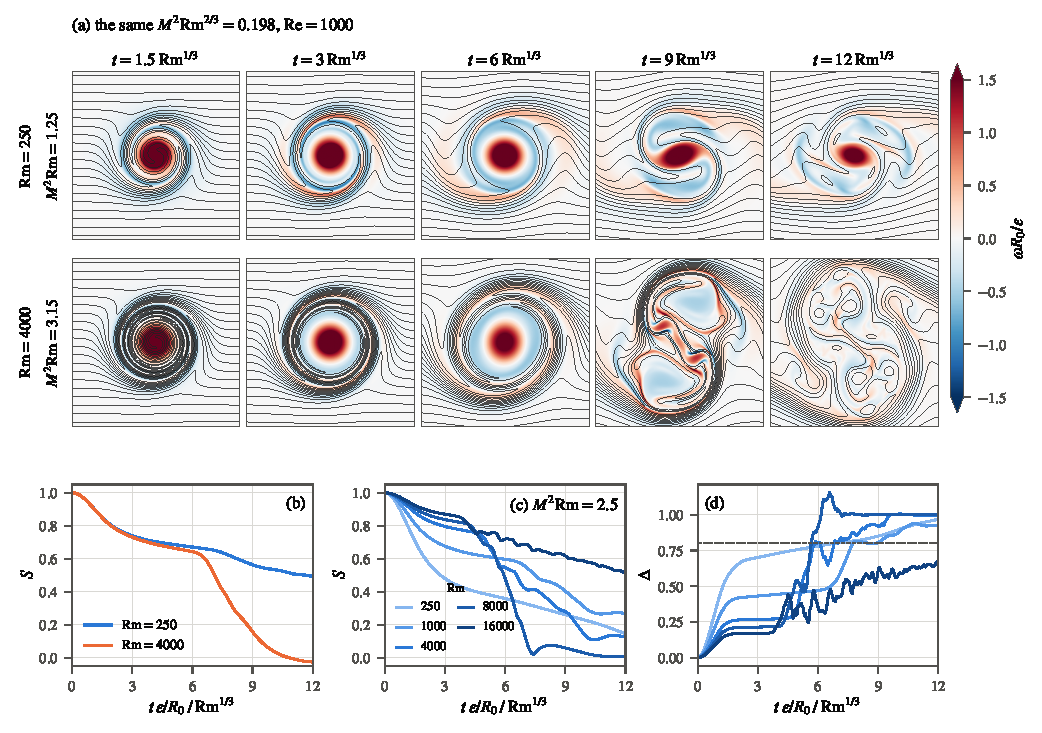
\includegraphics[width=\textwidth]{fig_pair}
\caption{(a) The same braking, two fates: vortices with the same
$M^2\Rm^{2/3}=0.198$ at $\Rm=250$ ($M^2\Rm=1.25$) and $\Rm=4000$ ($M^2\Rm=3.15$),
both at $\Rey=1000$ ($R_0=40$ cells), at the same times in units of
$\Rm^{1/3}$, and their survival $S$ (lower left). Colour: vorticity; lines:
magnetic field lines, contours of the flux function every $0.5B_0R_0$; the central
$10R_0$ of the $20R_0$ box. (b) One field, $M^2\Rm=2.5$, at $\Rm=\Rey=250$, $1000$,
$4000$, $8000$ and $16\,000$: $S$ and $\Delta$ against $t/\Rm^{1/3}$; dashed,
$\Delta=0.8$.}
\label{fig:pair}
\end{figure*}

\begin{figure}[!tb]
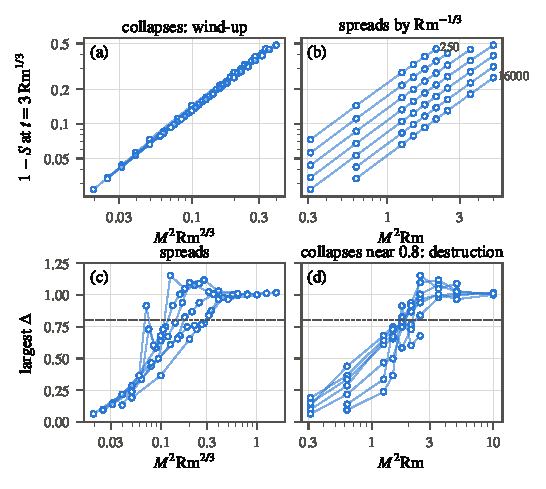
\includegraphics[width=\columnwidth]{fig_collapse}
\caption{(a,b) The braking during the wind-up, $1-S$ at $t=3\Rm^{1/3}$, against
$M^2\Rm^{2/3}$ and $M^2\Rm$. (c,d) The destruction, the largest $\Delta$ in the
run, against the same. Lines join the runs of one $\Rm$, from 250 to
$16\,000$. The dashed line is the threshold $\Delta=0.8$.}
\label{fig:collapse}
\end{figure}

\begin{figure}[!tb]
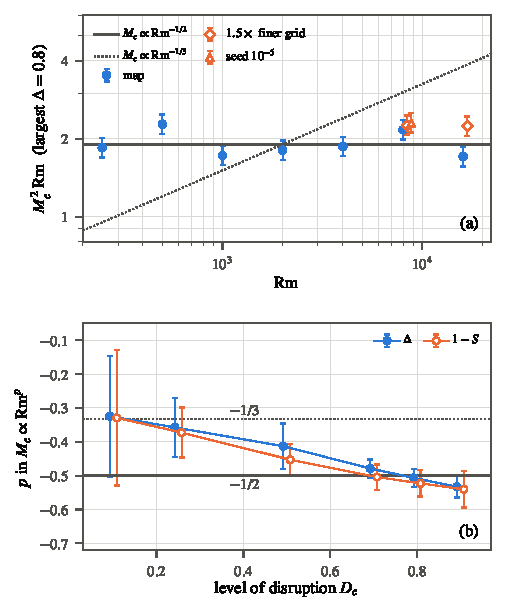
\includegraphics[width=\columnwidth]{fig_threshold}
\caption{(a) $M_c^2\Rm$ for destruction, $\Delta=0.8$, against $\Rm$. Error bars:
the field spacing. Diamonds: a grid 1.5 times finer; triangle: runs perturbed by
an ellipticity of $10^{-5}$. Lines: $M_c\propto\Rm^{-1/2}$ (solid) and
$\Rm^{-1/3}$ (dotted), through the mean of the map. (b) The exponent $p$ against
the level $D_c$
called a threshold, for $\Delta$ (filled) and $1-S$ (open); bars are the spacing
bound. Points are offset slightly in $D_c$.}
\label{fig:threshold}
\end{figure}

Here we follow a single vortex over a factor of 64 in $\Rm$ and find that both
scalings hold, for two different things. The braking of the vortex during the
wind-up grows as $M^2\Rm^{2/3}$; its destruction, which comes later and is
non-axisymmetric, needs $M^2\Rm\approx2$.

\textit{Setup.}---The vortex is the one whose stream function is a Gaussian,
\begin{equation}
u_\theta(r)=\eps\,\frac{r}{R_0}\exp\!\left[\frac{1}{2}\left(1-\frac{r^2}{R_0^2}\right)\right],
\label{eq:vortex}
\end{equation}
with peak speed $\eps$ at $r=R_0$ and no net circulation: its core is surrounded by
a ring of opposite vorticity. It sits at the centre of a periodic square of side
$20R_0$ in a uniform field $B_0\hat{\bm x}$. With the field in velocity units,
$M=B_0/\eps$, $\Rey=\eps R_0/\nu$ and $\Rm=\eps R_0/\eta$, and time is in units of
$R_0/\eps$. The magnetic Prandtl number is one except where stated. We solve the
two-dimensional MHD equations by the lattice Boltzmann method on the D3Q27
lattice for the flow and D3Q7 for the field, with one node in the third
direction. The flow uses a central-moment collision \cite{derosis2018} and the
field is carried as Dellar's vector distribution \cite{dellar2002}; we run at
$\eps=0.05$ lattice units (Mach number $0.087$) in double precision and seed the
density with the vortex's own pressure. Two codes that share no source implement
this, one of them in CUDA. Every run below is from the CUDA code except the one
that switches the field off, which only the other can do; the two agree to all
ten printed digits on a short run, and to $9.3\times10^{-10}$ of each diagnostic's
scale over a whole destruction run ($\Rey=\Rm=2000$, $M^2\Rm=2.5$, $t=0$--$151$).

Without the Lorentz force Eq.~\eqref{eq:vortex} is an exact viscous solution: its
vorticity, the Laplacian of a Gaussian, only spreads, and its projection on the
initial flow is $(1+t/\Rey)^{-2}$. We therefore measure what the field takes beyond
viscosity by
\begin{equation}
S(t)=\frac{\langle\bm u\cdot\bm u_0\rangle}{\langle\bm u_0\cdot\bm u_0\rangle}\,(1+t/\Rey)^{2},
\end{equation}
which is 1 for a vortex the field has not touched. A run without the force
recovers the set viscosity to $0.9990$ and keeps $|S-1|\le1.8\times10^{-4}$. The
second measure is built from velocity gradients, after Mak \textit{et al.}: with
$W=s^2-\omega^2$ the Okubo--Weiss parameter \cite{okubo1970,weiss1991},
$\Delta=1-\int_A W\big/\int_A W_\mathrm{ref}$, where $W_\mathrm{ref}$ is that of the
exact viscous vortex at the same time and $A$ the region where
$W_\mathrm{ref}<-0.2$ times its root-mean-square value. $\Delta=0$ for an intact
vortex and $\Delta\gtrsim1$ once strain has replaced rotation where the core was.
Unlike Ref.~\cite{mak2017} we fix $A$ by the reference rather than by the run's own
largest rotation-dominated patch, so the two $\Delta$ are not comparable number for
number.

The map covers $\Rm=\Rey=250$, 500, 1000, 2000, 4000, 8000 and $16\,000$, at
$R_0=20$ cells up to $\Rm=4000$, 40 at 8000 and 80 at $16\,000$, which keeps the
relaxation times at least $7.5\times10^{-4}$ above their stability limit of
$1/2$. Each $\Rm$ has eight fields from $M^2\Rm=0.625$ to $5$, a factor 1.09
apart in $M$ near the threshold, and up to $\Rm=4000$ two more, $0.3125$ and
$10$. Every run lasts $t=12\Rm^{1/3}$; two of the 66 went non-finite, both at
$\Rm=16\,000$ and above the destruction threshold ($M^2\Rm=3.54$ and $5$).

\textit{Two stages.}---Figure~\ref{fig:pair}(a) puts the result in one picture. The
two vortices have the same $M^2\Rm^{2/3}$ and, as shown below, therefore the same
braking: the vortex winds the field into a spiral and expels it from its core, and
their survival curves agree within $0.022$ up to $t=5\Rm^{1/3}$. Then they part.
At $\Rm=4000$, where $M^2\Rm=3.15$ is above the destruction threshold, the core is
drawn into an elongated vortex with two satellites, a tripole, and torn apart,
with $S=-0.026$ at the end; at $\Rm=250$, where $M^2\Rm=1.25$ is below it, the
core is eroded but not destroyed, with $S=0.493$ and $\Delta=0.708$ at the end.
Figure~\ref{fig:pair}(b) follows one field across
$\Rm=250$--$16\,000$. During the wind-up $\Delta$ rises to a plateau that falls with
$\Rm$, from $0.701$ at $\Rm=250$ to $0.170$ at $\Rm=16\,000$ at $t=3\Rm^{1/3}$; on
the weakest row, $M^2\Rm=0.3125$, the peak field reaches
$1.04$--$1.10\,\Rm^{1/3}B_0$. From $\Rm=1000$ up a second, separate rise follows
the plateau. At $\Rm=250$ the two merge into a steady erosion: the vortex is
sheared away during the wind-up itself, without a tripole (Figs.~S1--S3 of the
Supplemental Material). And a tripole is not by itself destruction: at
$\Rm=4000$ and $M^2\Rm=1.25$ one forms, but the largest $\Delta$ is $0.47$ and the
core recovers, $\Delta$ falling to $0.311$ by the end (Fig.~S1).

\textit{Braking.}---Read at $t=3\Rm^{1/3}$, near the peak of the wound field,
$1-S$ along each row of fixed $M^2\Rm$ falls as $\Rm^q$ with $q=-0.337$ to
$-0.359$ on the six rows with $M^2\Rm\le2.1$, and $\Delta$ gives $q=-0.350$ to
$-0.400$. (Above them the braking is no longer small and $q$ flattens, to
$-0.305$ at $M^2\Rm=5$ and $-0.166$ at $10$.) A dependence on $M^2\Rm$ alone would
give $q=0$; one on $M^2\Rm^{2/3}$ gives $q=-1/3$. The braking therefore collapses on
$M^2\Rm^{2/3}$ [Fig.~\ref{fig:collapse}(a)] and not on $M^2\Rm$
[Fig.~\ref{fig:collapse}(b)]: $1-S=(1.33$--$1.47)\,M^2\Rm^{2/3}$ over the 19 runs
with $M^2\Rm\le1.25$. This reading is converged: a grid 1.5 times finer, at
$\Rm=250$--$16\,000$, changes $1-S$ by at most $0.31\%$ and $\Delta$ by at most
$0.62\%$. It is the scaling
Gilbert \textit{et al.} \cite{gilbert2016} found for the onset of the dynamical
regime with an axisymmetric flow, and in this stage the vortex stays axisymmetric
[Fig.~\ref{fig:pair}(a)].

\textit{Destruction.}---Defining the vortex as destroyed when $\Delta$ reaches
$0.8$, and $M_c$ as the field that does it, interpolated in $\ln M$ between the
two runs that bracket it, we find $M_c^2\Rm=1.70$--$2.27$ at all seven $\Rm$
from 250 to $16\,000$ [Figs.~\ref{fig:collapse}(d) and
\ref{fig:threshold}(a)]. For the runs at $\Rm=2000$--$16\,000$ we fixed the rule
before they ran: fitting $M_c\propto\Rm^p$, $p$ is uncertain by the largest of
the spacing bound ($0.050$), the shift when the thresholds at $\Rm=8000$ and
$16\,000$ are taken from a grid $1.5$ times finer ($0.061$), and the shift when the
threshold at $\Rm=8000$ is taken from runs perturbed by an ellipticity of $10^{-5}$
($0.004$). It gives $p=-0.502\pm0.061$, excluding $-1/3$ by $0.168$. The same
rule over all seven $\Rm$ gives $p=-0.507\pm0.027$, excluding $-1/3$ by $0.173$.

The exponent depends on how much disruption is called a threshold
[Fig.~\ref{fig:threshold}(b)]. For $\Delta$ it is $-0.357$, $-0.413$, $-0.479$,
$-0.507$ and $-0.533$ at $D_c=0.25$, $0.5$, $0.7$, $0.8$ and $0.9$ (and
$-0.33\pm0.18$ at $0.1$, which only three $\Rm$ reach), and $1-S$ steepens the
same way, from $-0.373$ at $0.25$ to $-0.504$, $-0.523$ and $-0.540$ from $0.7$
up.
A low level is reached during the wind-up and inherits its scaling; only
destruction needs the second stage. The $-1/2$ is a statement about destruction,
not about every threshold.

Because $\Rm^{-1/2}$ falls faster than $\Rm^{-1/3}$, the field that destroys a
vortex brakes it less and less during the wind-up as $\Rm$ rises. Along
$M^2\Rm=2.10$, next to the threshold, $1-S$ at $t=3\Rm^{1/3}$ falls from $0.448$ at
$\Rm=250$ to $0.110$ at $\Rm=16\,000$, as $\Rm^{-0.34}$. At large $\Rm$ destruction is
not the end point of braking; it is a separate, non-axisymmetric instability that a
model with an axisymmetric flow cannot contain.

\textit{The second stage is the field's.}---Vortices with a shielding ring can
form tripoles by themselves \cite{carton1989}, so we checked that this one does not
within the time we follow. At $\Rey=\Rm=2000$ without the Lorentz force, a $1\%$
elliptical perturbation leaves $S=0.9968$ at $t=151$. With the field at
$M^2\Rm=2.5$ the vortex is still axisymmetric at $t=50$ ($S=0.713$) and is gone by
$t=126$ ($S=-0.054$). Removing the field at $t=50$, after the wind-up, the vortex
dips to $S=0.590$ at $t=82$ and recovers to $0.674$. Destruction therefore needs
the field to keep acting during the second stage. That is the picture behind Mak
\textit{et al.}'s estimate \cite{mak2017}, in which the curl of the tension of the
wound field, $M^2J(A,\nabla^2A)$ in the vorticity equation, grows as $M^2\Rm$ in
units of $\eps^2/R_0^2$ and disrupts the vortex when it rivals the vortex's own
advection. We have tested the outcome of that estimate, not its intermediate
steps.

\textit{Magnetic, not viscous.}---The maps move $\Rey$ with $\Rm$. Two slices through
$\Rey=\Rm=1000$ separate them. With $\Rey=1000$ and $\Rm=250$--$4000$ the braking
gives $q=-0.324$ and the destruction $p=-0.468\pm0.038$; with $\Rm=1000$ and
$\Rey=250$--$4000$, $q=-0.040$ and $p=-0.065\pm0.038$. Both scalings belong to
$\Rm$. What viscosity adds is a residue at low $\Rey$: $M_c^2\Rm=2.38$ at
$\Rey=250$ against $1.66$--$1.72$ for $\Rey\ge1000$.

\textit{Caveats.}---First, the threshold is destruction within $t=12\Rm^{1/3}$, and
destruction comes later in that window as $\Rm$ rises: at $M^2\Rm=2.5$ the largest
$\Delta$ is $1.153$ at $0.55$ of the window for $\Rm=8000$, but only $0.678$ at its
end for $\Rm=16\,000$, where four of the five runs bracketing the threshold reach
their largest $\Delta$ in the window's last tenth. A shorter window can only raise
$M_c$, and it raises it most at the largest $\Rm$, so the truncation makes $p$
shallower: it cannot have turned a $-1/3$ into the $-1/2$ we measure. Second, the second stage is chaotic: an ellipticity of $10^{-5}$ changes
the largest $\Delta$ of a single run by up to $0.213$, and along $\Rm=8000$ the
largest $\Delta$ is not monotonic in $M$. The finer grid moves $M_c$ at
$\Rm=16\,000$ by $+14.4\%$ through one run whose neighbours shift the other way.
Both effects are inside the quoted uncertainty, which was defined to contain them.
Third, this is one vortex profile, in two dimensions, at unit magnetic Prandtl
number apart from the two slices.

\textit{Conclusion.}---The two criteria in the literature are both right, for
different things. $M^2\Rm^{2/3}$ measures how much the wound field brakes a vortex;
$M^2\Rm$, near 2, decides whether it is destroyed. If these scalings persist, at
astrophysical $\Rm$ the field that destroys a vortex is smaller than the one that
would visibly brake it by $\Rm^{1/6}$, a factor of 100 at $\Rm=10^{12}$, and a
vortex can disappear from a weakly magnetized flow without first slowing down.

\begin{acknowledgments}
% TODO(author): funding; APS asks that any use of AI tools in preparing the
% manuscript be disclosed (this draft was prepared with one).
The code and the series behind every figure are at
\url{https://github.com/alexderosis/M3LB}.
\end{acknowledgments}

\bibliography{refs}

\end{document}
